\section{Approfondimenti}
\subsection{Copy-on-write}

\subsubsection{Introduzione}
	Copy-on-write (CoW o COW), spesso noto anche come \textbf{shadowing} o \textbf{implicit 
	sharing}, e' una tecnica di gestione delle risorse utilizzata nell'informatica per 
	implementare in maniera efficiente le operazioni di "duplicazione" o "copia" su risorse 
	soggette a modifiche. Se una risorsa e' duplicata ma non modificata, non e' necessario 
	creare una nuova risorsa (la copia); la risorsa puo' infatti essere condivisa fra la copia e 
	l'originale. Eventuali modifiche pero' devono comunque creare una copia, da qui' la tecnica:

	\subparagraph{Tecnica}
		L'effettiva operazione di copia viene 'rinviata' alla prima scrittura sulla risorsa. 
		Condividendo le risorse in questo modo, e' possibile ridurre in modo significativo il 
		consumo di risorse di dovuto a copie non modificate, aggiungendo un piccolo sovraccarico 
		alle operazioni di modifica delle risorse.

\subsubsection{VirtualBox}
	VirtualBox puo' avvalersi di snapshot per congelare lo stato di un disco virtuale.

	\subparagraph{Utilizzo originale}
		Utilizzato per backup coerenti 'a caldo' con Copy-on-write.
		\begin{itemize}
			\item Creo un disco virtuale 'snapshot'
			\item Lascio che i processi del S.O. lavorino sul disco originale
			\item Do l'illusione alla procedura di backup che legge dallo snapshot che nessuno 
			stia modificando il disco
		\end{itemize}

		\begin{figure}[H]
			\centering
			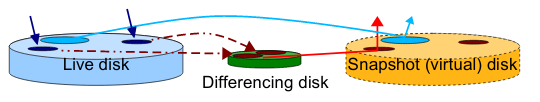
\includegraphics[scale=0.8]{img/approfondimenti-vbcow.png}
			\caption{Ogni scrittura sul disco live provoca il salvataggio del settore originale 	
			sullo spazio di appoggio dello snapshot (differencing disk) }

			\begin{itemize}
					\item I settori copiati vengono enumerati in una exeption table
					\item La lettura sullo snapshot disk di un settore \textbf{modificato} viene 
					fatta dal \textbf{differencing disk}
					\item La lettura sullo snapshot disk di un settore \textbf{non modificato} 
					viene fatta dal \textbf{live disk}
			\end{itemize}

		\end{figure}
	
	\subparagraph{VirtualBox Snapshot}
		Utilizzato per la condivisione dello storage tra piu' macchine virtuali simili
			\begin{itemize}
				\item Installo una VM 'base' su un disco che dichiaro immutabile
				\item Utilizzo quel disco come device per altre VM						
			\end{itemize}	

			\begin{figure}[H]
				\centering
				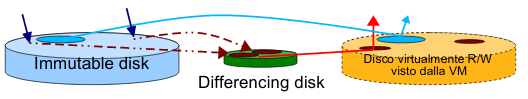
\includegraphics[scale=0.8]{img/approfondimenti-vbcow1.png}
				\caption{Per ogni VM viene allocato un differencing disk di appoggio; ogni 
				scrittura sul disco immutabile viene in realta' eseguita sul differencing disk}

				\begin{itemize}
					\item I settori corrispondenti vengono enumerati in una exeption table
					\item La lettura di un settore \textbf{modificato} viene fatta dal 			
					\textbf{differencing disk}
					\item La lettura di un settore \textbf{non modificato}	 
					viene fatta dal \textbf{live disk}
				\end{itemize}

			\end{figure}

\subsection{VirtualBox Configuration}
	\subsubsection{Machine Registry}
	VirtualBox ha un Machine Registry dove elenca le VM note e alcuni parametri di configurazione
	globali. E' possibile trovare questi in file in \texttt{~/.config/VirtualBox/VirtualBox.xml}.
	Tra questi parametri globali e' presenta la directory di default per la creazione delle macchine
	virtuali.

	\subsubsection{Media Registry}
	Nel file \texttt{.vbox} e' definito un indice di risorse relative alla macchina virtuale in oggetto
	noto come Media Registry. Nel caso di macchine create come \textit{linked clone}, le immagini
	disco sono in realta' snapshot del disco base, quindi sono tutte definite nel file di configurazione
	della macchina di base.
	
	\begin{figure}[H]
		\centering
		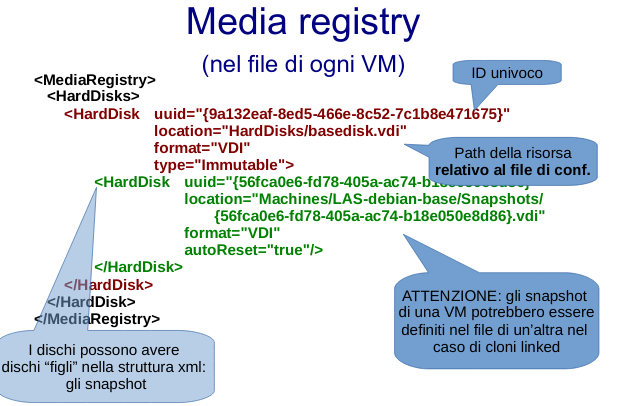
\includegraphics[scale=0.8]{img/media_registry.png}
		\caption{Struttura di un Media Registry}
	\end{figure}

\subsection{Filesystem}\label{filesystem}
TODO.



